\chapterimage{estados.jpg} % Table of contents heading image
\chapter{Estados}

Un estado es una situación durante la vida de un objeto, de forma que cuando dicha situación se satisface se lleva a cabo alguna acción o se espera por un evento. El estado de un objeto se puede caracterizar por el valor de una o varias de las características de su clase, además, el estado de un objeto también se puede caracterizar por la existencia de un enlace con otro objeto. El diagrama de estados y transiciones incluye todos los mensajes que un objeto puede enviar o recibir. En un diagrama de estados, un escenario simboliza un camino dentro del diagrama. Dado que generalmente el espacio entre dos envíos de mensajes representa un estado, se pueden utilizar los diagramas de secuencia para buscar los diferentes estados de un objeto \cite{Pw5DE}.

Nuestro software posee elementos que tiene diferentes estados, para poder observar como estos estados cambian, y cuales son las condiciones de transición entre estos, de mostrará a continuación un diagrama de estados donde se resume todo esto.

\section{Diagrama de Estados}

Los diagramas de estado son un método conocido para explicar el comportamiento de un sistema. Que explican todos los estados posibles en los que puede ingresar un objeto particular y la manera en que modifica el estado del objeto, como resultado de los eventos que llegan a el. Permite identificar bajo qué pruebas se ejecuta cada uno de los procesos y en qué momento podrían tener una variación. El diagrama de estados permite visualizar de una forma ordenada la ejecución de cada uno de los procesos \cite{Pw5DE}.

La figura mostrada a continuación tiene el diagrama de estados del ciclo de vida que sufre la clase FlujoEconomico la cual puede encontrarse en tres diferentes estados, ACTIVO, EN ESPERA y FINALIZADO. El disparo a nivel general es la operación verificarTiempo la cual recibe como parámetro un tiempoActual, y es una referencia para poder realizar comparaciones y establecer así el efecto que se lleva acabo de forma determinada. Ahora bien, existen tres transiciones entre cada fase:

Desde el estado ACTIVO hacia el estado EN ESPERA la condición es que el tiempoActual sea diferente el tiempoDeEjecucion y que sea de naturaleza cíclica para poder pasar al efecto de suspender.

Desde el estado EN ESPERA hacia el estado ACTIVO la condición es que el tiempoActual sea igual al tiempoDeEjecucion y cuyo efecto es el de notificar.

Desde el estado ACTIVO a FINALIZADO la condición es que es que el tiempoActual sea mayor al tiempoDeEjecución y no sea ciclico para desembocar en el efecto de finalizar.

\begin{figure}[H]
	\centering
	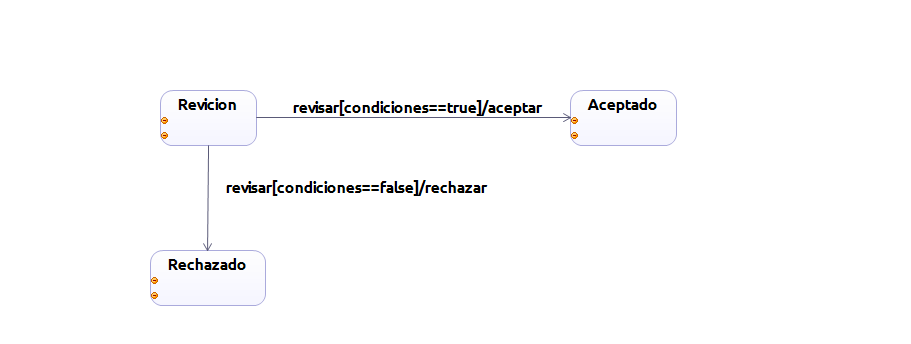
\includegraphics[width=1\linewidth]{parte2/imgs/DiagramaDeEstado/estados}
	\caption{Diagrama de Estado}
	\label{fig:diagramaEstado}
\end{figure}

\paragraph{Diagrama de clases} 

En el siguiente esquema se muestra la clase foco que es FlujoEconomico, ésta es la que cambia de estados según las condiciones dadas, para ello debe tener como atributos un ESTADO, que es el que va a variar, y los métodos necesarios para actuar a la hora de cambiar de estado.

\begin{figure}[H]
	\centering
	\includegraphics[width=1\linewidth]{parte2/imgs/DiagramaDeEstado/clase}
	\caption{Diagrama de Clase FlujoEconomico}
	\label{fig:diagramaEstadoClase}
\end{figure}

\paragraph{Código}

El siguiente es código de nuestra clase, éste es generado por el programa de software Coloso, para la generación de éste se involucra el panorama de Java y sirve como plantilla para generar la clase correspondiente.

\begin{figure}[H]
	\centering
	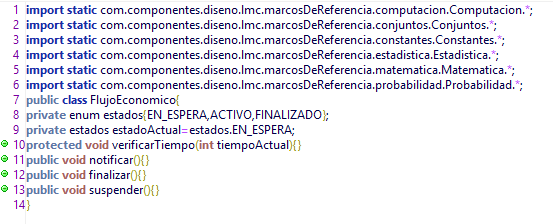
\includegraphics[width=1\linewidth]{parte2/imgs/DiagramaDeEstado/codigo}
	\caption{código de Clase FlujoEconomico}
	\label{fig:diagramaEstadoClaseCodigo}
\end{figure}\newpage

%%%%%%%%%%%%%%%%%%%%%% Seccion 5.2 %%%%%%%%%%%%%%%%%%%%%%%%%%%%%
\section{Diagrama de flujo de trabajo}
Los diagramas de flujo de trabajo describen el comportamiento del sistema cuando tiene una actividad lo suficientemente grande para requerir un detallado de ésta, de las partes y de cómo interactuan entre sí.

Para desarrollarlo se implementan diferentes elementos como:

\begin{itemize}
	\item \textbf{Particiones}: Es una abstracción de las partes del sistema que interactua entre sí.
	\item \textbf{Actividades}: Son las tareas que le corresponde realizar a cada partición.
	\item \textbf{Transiciones}: Dan el orden en que las particiones deben desarrollar sus tareas siendo cada una dependiente de la anterior.	
	\item \textbf{Estado final}: Es el estado al que debe llegar el flujo cuando se culmine el proceso y no hayan más transiciones.
\end{itemize}

Para el software de EconomApp podemos encontrar, entre sus diferentes actividades, dos actividades relevantes: Inserción de un flujo a la base de datos y Selección de sugerencias, estas tienen un grado de complejidad mayor al resto de actividades y por ello a continuación se describirán los flujos de trabajo para cada uno.

\paragraph{Inserción de un flujo a la base de datos}

La inserción de un nuevo flujo económico exige la abstracción de tres particiones, el usuario, la plataforma y la persistencia, los cuales se relacionan de forma que , cuando el usuario quiera añadir nuevos flujos económicos tenga la capacidad de visualizar aquellos que ya existen, y llegado el caso que encuentre uno similar, solicite a la plataforma, ya sea diferenciarlo del que se encontró debido a que es estrictamente necesario añadirlo o simplemente darse cuenta que no necesita añadir uno nuevo y cancelar la operación. 

\begin{figure}[H]
	\centering
	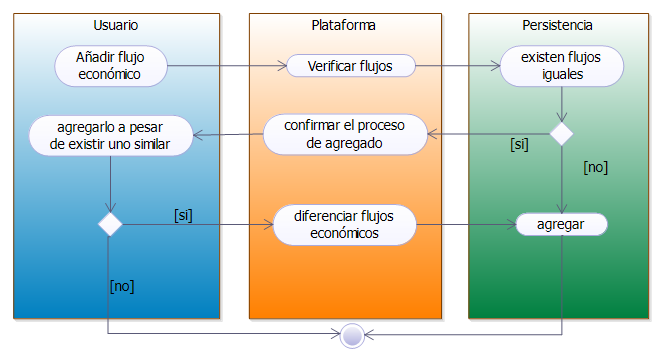
\includegraphics[width=1\linewidth]{parte2/imgs/DiagramaDeFlujoDeTrabajo/DiagaramaDeFlujo1}
	\caption{Diagrama de flujo de trabajo para agregar un flujo nuevo}
	\label{fig:workflowAgregarFlujo}
\end{figure}

\paragraph{Selección de sugerencias}
	
Las sugerencias se realizan automáticamente teniendo en cuenta un flujo económico particular, por lo que la plataforma debe solicitar a la persistencia los flujos existentes para seleccionar uno, evaluar sus características y poder hacer la creación. Ahora bien, estas sugerencias son mostradas al usuario para que éste tome la decisión de guardarla o simplemente ignorarla. Terminado el proceso de selección, la plataforma, consciente de las sugerencias seleccionadas interactua con la persistencia para guardarlas y ella misma notifica al usuario finalmente.
	
\begin{figure}[H]
	\centering
	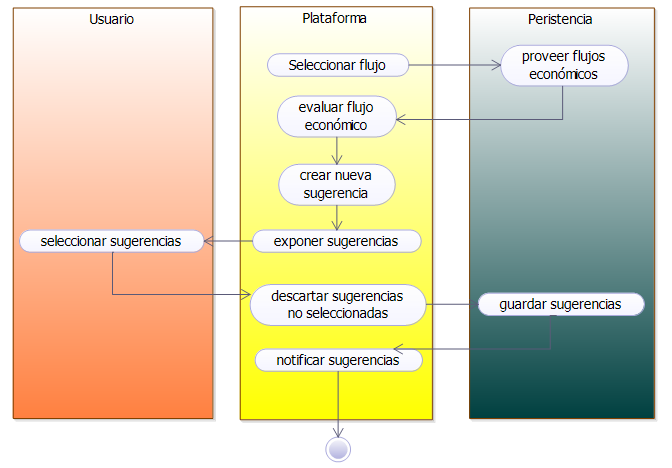
\includegraphics[width=1\linewidth]{parte2/imgs/DiagramaDeFlujoDeTrabajo/DiagramaDeFlujo2}
	\caption{Diagrama de Flujo de trabajo para la selección de sugerencias}
	\label{fig:diagramaSeleccionarSugerencias}
\end{figure}